\newpage
\section{Materials database}
\label{sec:materialdatabase}
Related YouTube videos:
\begin{figure}[H]

\begin{tabular}{ c l }


\includegraphics[width=0.05\textwidth]{./images/youtube.png}

&
\href{https://www.youtube.com/watch?v=0u6_jRVhZwU}{A tutorial on adding new materials to OghmaNano}

\end{tabular}
\end{figure}

This database primarily contains n/k data and PL emission spectra. However it also contains some electrical information and some thermal information. Each subdirectory within the materials database identifies the material name.  In each sub directory there are two key files $alpha.csv$ and $n.csv$, these files are standard text files can be opened with any text editor such as wordpad.  Alpha.csv contains the absorption coefficient of the material while n.csv contains the the refractive index.  The first column of the file contains the wavelength in $m$ (not $cm$ or $nm$), and the second column of the file contains the absorption coefficient in $m^{-1}$ (for alpha.csv) and the real part of the refractive index (i.e. n) in au (for n.csv). The data.json defines the material color and any known electrical or thermal data. If the material is used in emissive optical simulations the emission spectra of the material will be stored in a file called $emission.csv$. An example material directory, in this case Alq3 can be seen in figure \ref{fig:material_example}, a description of these files can be found in \ref{tab:db_item_files}.


\begin{figure}[H]
\centering
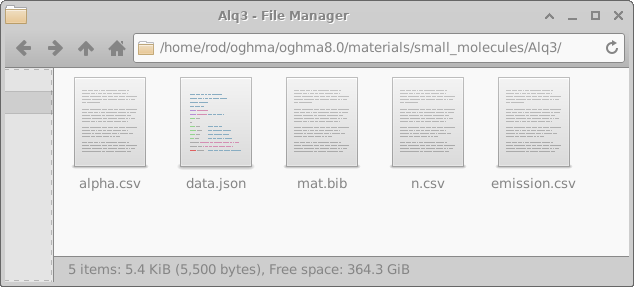
\includegraphics[height=0.18\textwidth]{./images/database_materials/db_item.png}
\caption{An example of a materials database item for Alq3.}
\label{fig:material_example}
\end{figure}

\begin{table}[H]
\begin{center}
\begin{tabular}{ |c|l|c| } 
 \hline
	File name 			& 	Description  \\ 
 \hline
	data.json			&	json file infomration about the material (LUMO/HOMO levels etc..) \\ 
	alpha.csv			&	wavelength (m) v.s. absorption ($m^{-1}$) \\ 
	n.csv 			&	wavelength (m) v.s. refractive index (au)\\ 
	$emission.csv^{*see below}$ 		&	wavelength (m) v.s. PL emission (au)\\
	mat.bib 			&	Bibtex file containing references\\ 
 \hline
\end{tabular}
\caption{A summary of the files making up each material in the materials database. *The file emssion.csv is not needed unless the material forms part of an emissive layer of an OLED or other such light emitting device.}
\label{tab:db_item_files}
\end{center}
\end{table}
\pagebreak

\subsection{Adding new materials - the hard way}
If you wish to add materials to the database which do not come as standard with the model you can do it in the following way:  Simply copy an existing material directory (say oghma\_local$\backslash$materials$\backslash$oxieds$\backslash$ito) to a new directory (say oghma\_local$\backslash$materials$\backslash$oxieds$\backslash$mynewmaterial).  Then replace alpha.csv and n.csv with your data for the new material. You can ignore the data.json file, although if you know the energy levels you can add the values in the file.

If you don't have data to hand for your material, but you do have a paper containing the data, you use the program Engauge Digitizer, written by  Mark Mitchell \url{https://github.com/markummitchell/engauge-digitizer} to export data from publications.  After you have finished updating the new material directory, whenever a new simulation is generated the new material files will automatically be copied into the active simulation directory ready for use.
\vspace*{\fill}
\pagebreak

\subsection{Adding new materials - the easy way}

To add a new material go to the database ribbon and click on \emph{Materials database} as shown in figure \ref{fig:materialadd1}.
\begin{figure}[H]
\centering
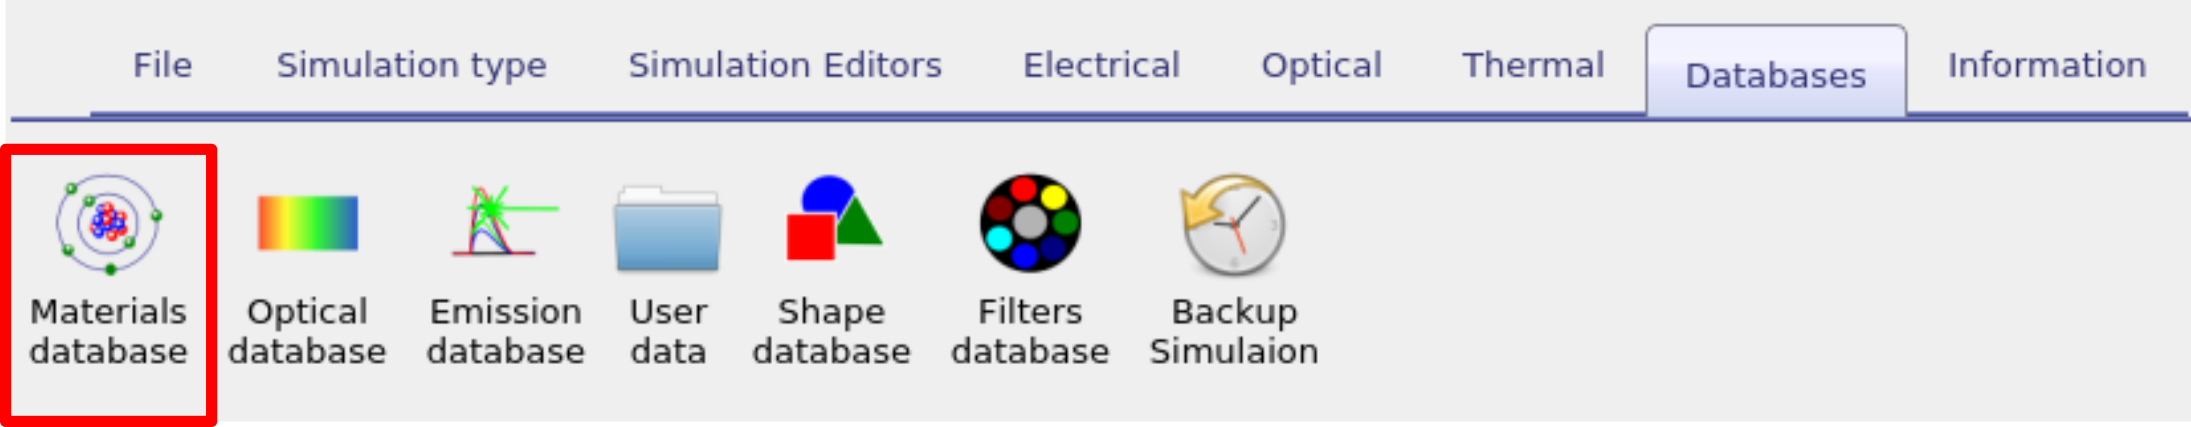
\includegraphics[height=0.18\textwidth]{./images/database_materials/database_materials.png}
\caption{Opening the materials database}
\label{fig:materialadd1}
\end{figure}

Then click \emph{add material} in the top right of the window, this will bring up a dialogue box which will ask you to give a name for your new material, this is visible in figure \ref{fig:materialadd3}. In this case we called the material my\_new\_material.

\begin{minipage}{0.5\textwidth}
	\centering
	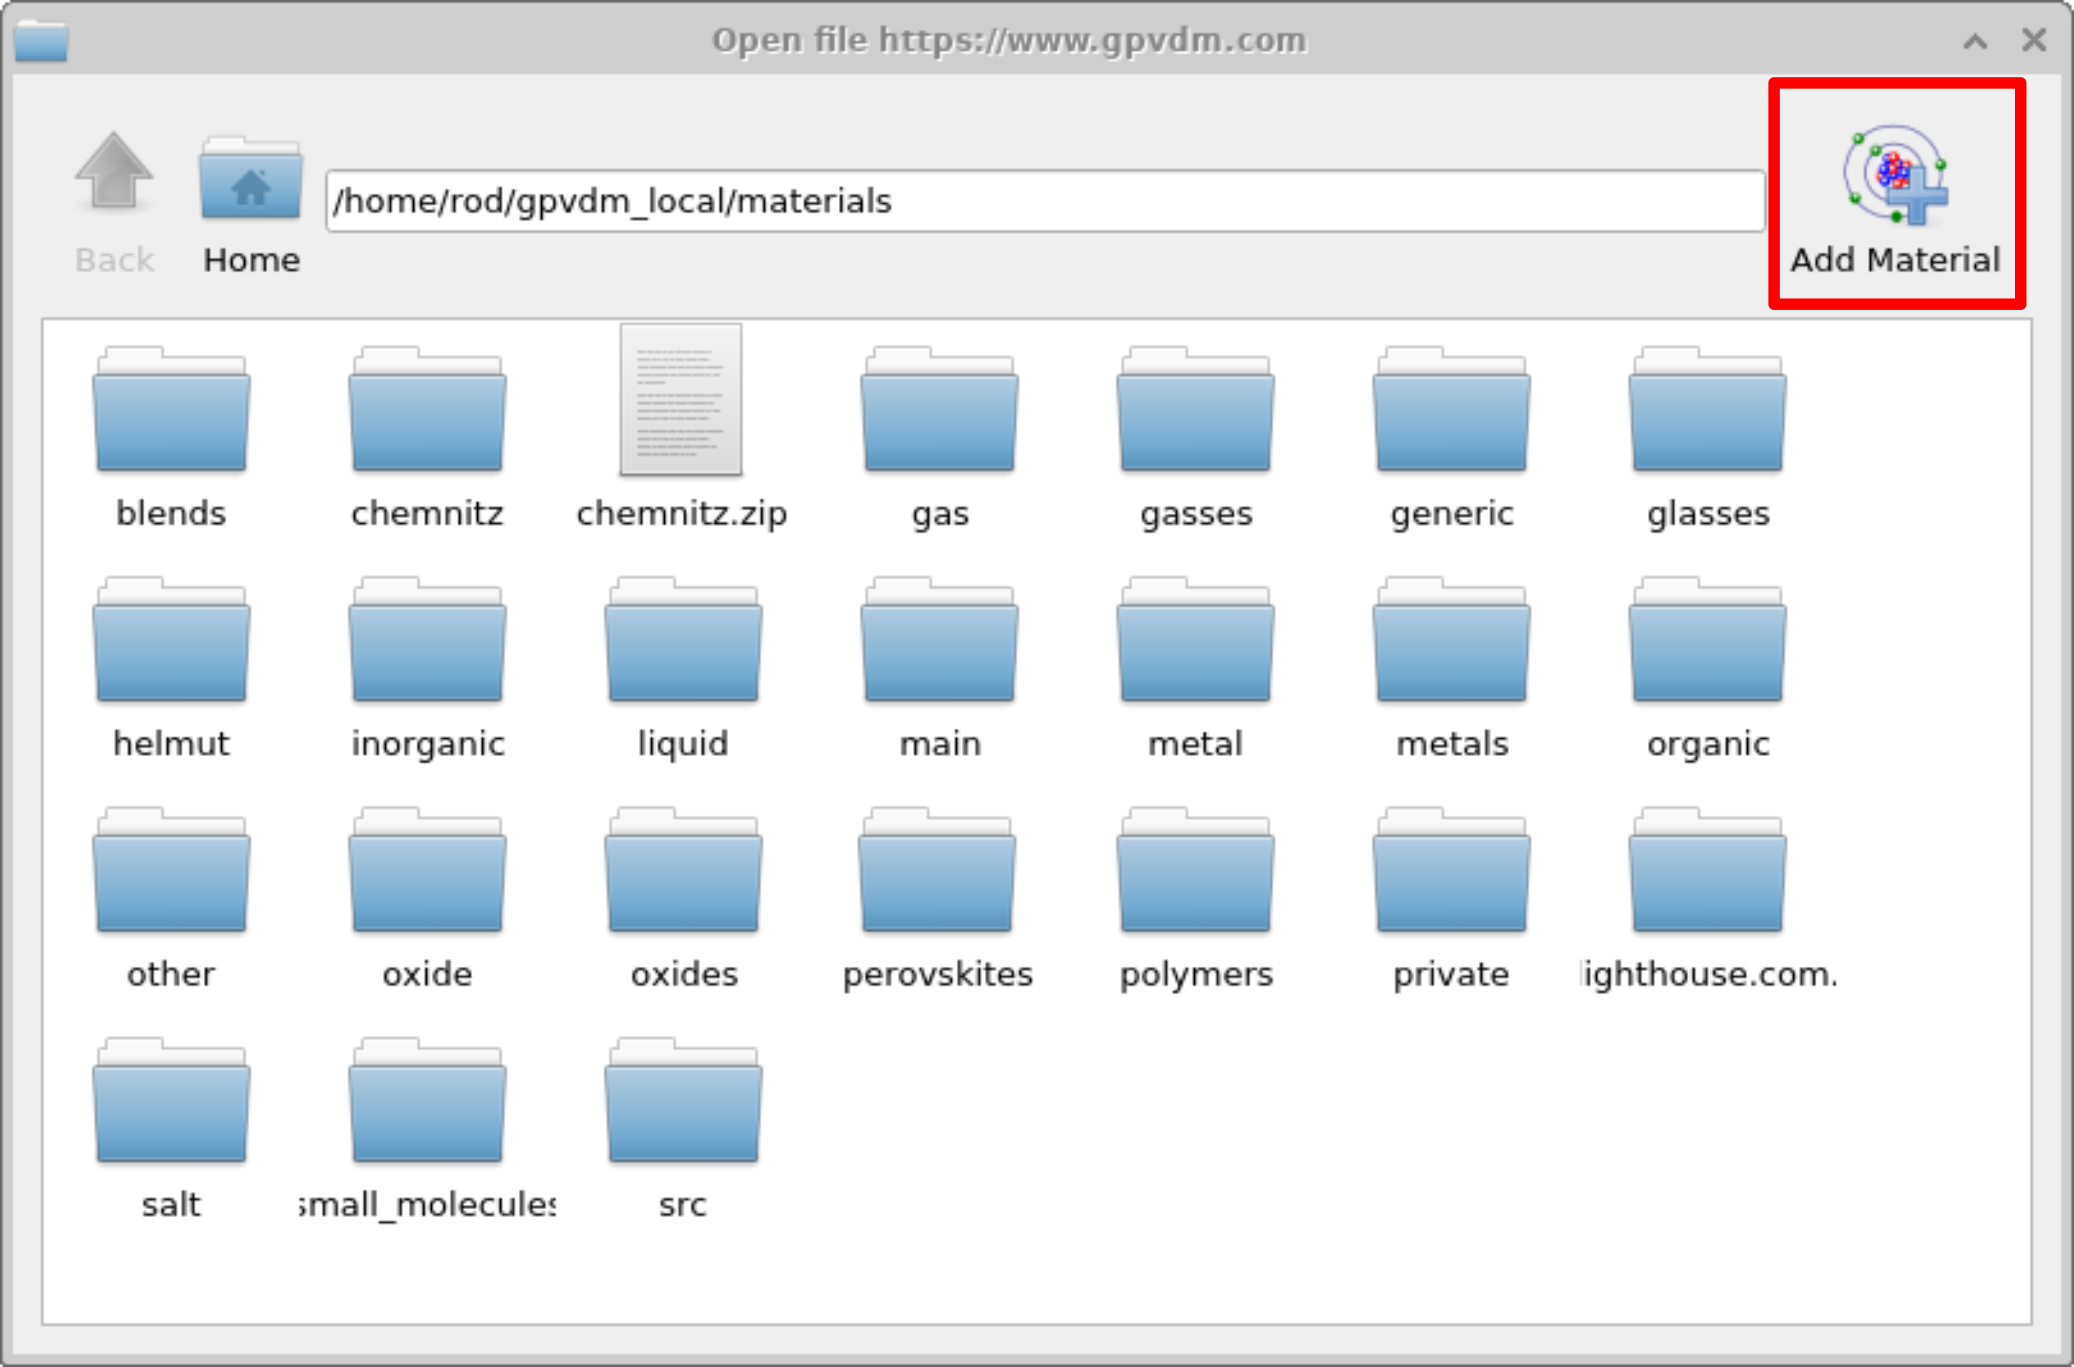
\includegraphics[width=\linewidth,height=0.8\linewidth]{./images/database_materials/database_materials_add.png}
	\captionof{figure}{Select Add material}
	\label{fig:materialadd2}
\end{minipage}
\hspace{4pt}
\begin{minipage}[]{0.5\linewidth}
	\centering
	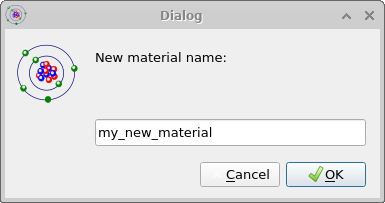
\includegraphics[width=\linewidth,height=0.6\linewidth]{./images/database_materials/database_materials_set_name.png}
	\captionof{figure}{Type the name of the new material}
	\label{fig:materialadd3}
\end{minipage}
Once you have clicked OK the new material will appear see Figure \ref{fig:materialadd4}, open it by double clicking on it. This will bring up an empty material window with no data. See Figure \ref{fig:materialadd5}.

\begin{minipage}{0.5\textwidth}
	\centering
	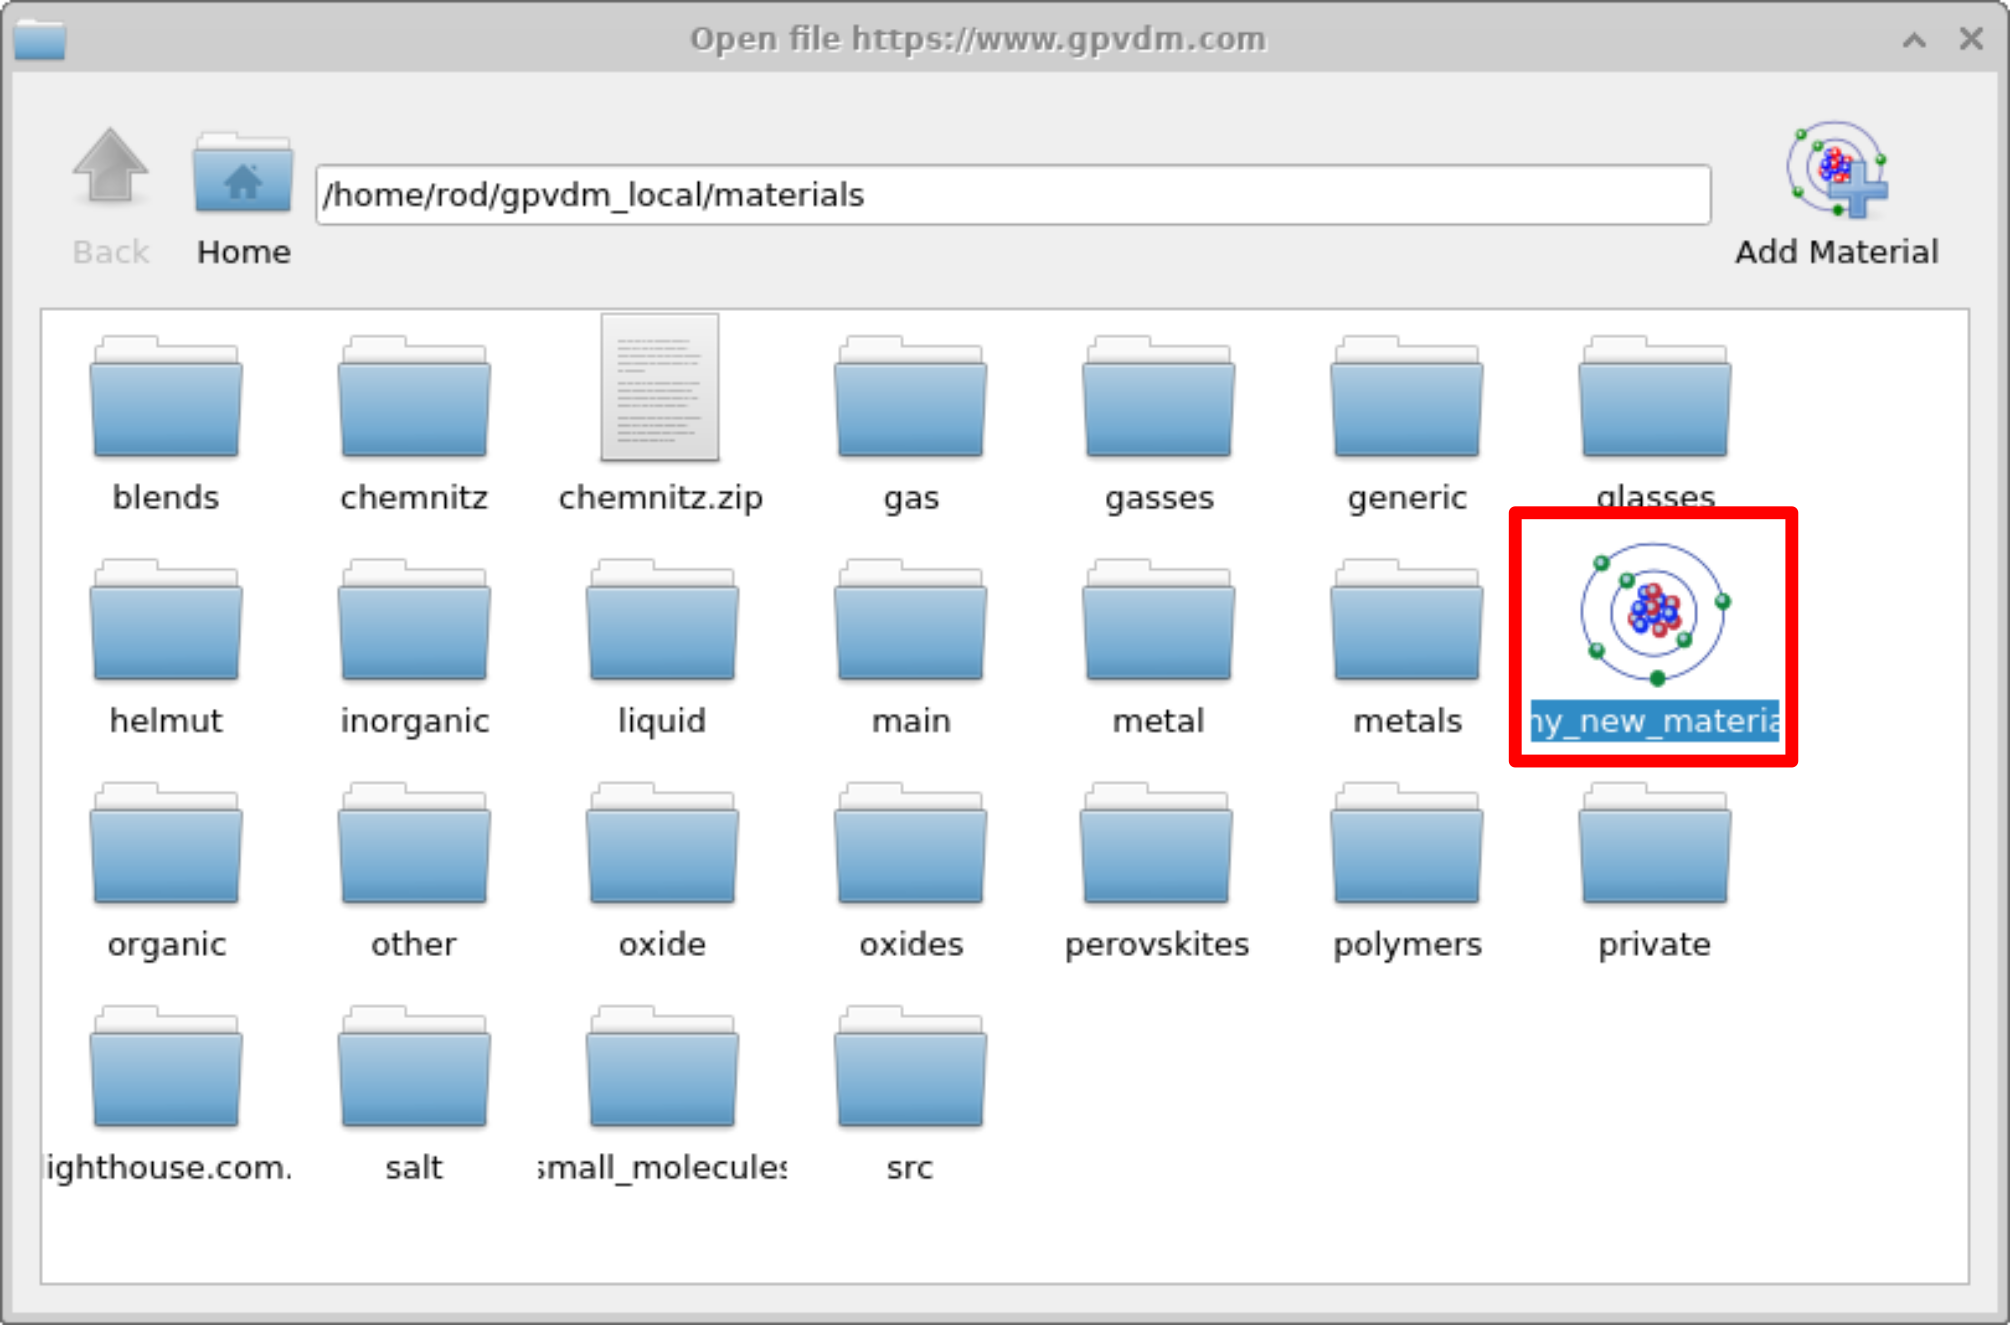
\includegraphics[width=\linewidth,height=0.8\linewidth]{./images/database_materials/database_materials_open.png}
	\captionof{figure}{Open the new material}
	\label{fig:materialadd4}
\end{minipage}
\hspace{4pt}
\begin{minipage}[]{0.5\linewidth}
	\centering
	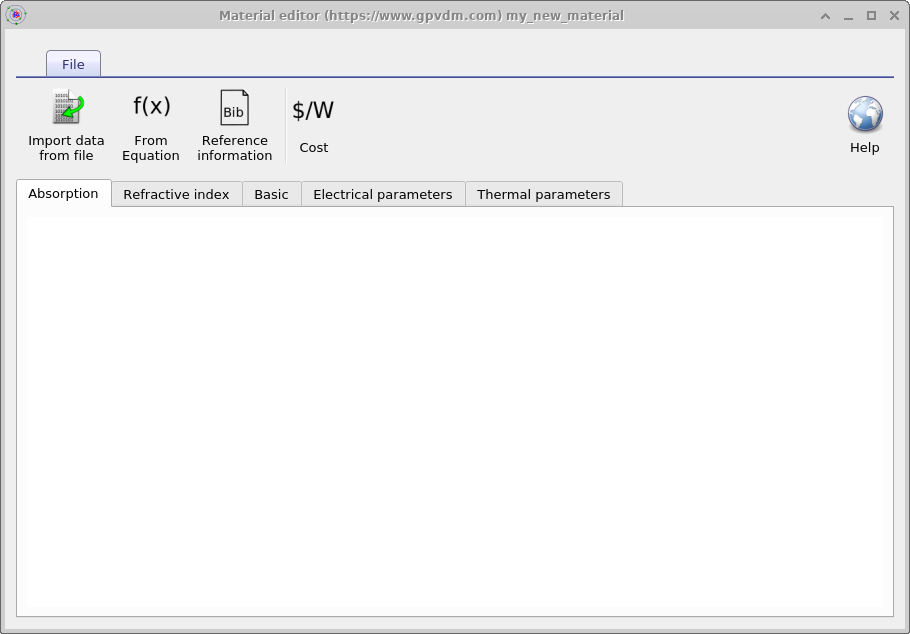
\includegraphics[width=\linewidth,height=0.6\linewidth]{./images/database_materials/database_window.png}
	\captionof{figure}{The new material without any data}
	\label{fig:materialadd5}
\end{minipage}

To import data to the material use the \emph{Import data from file} button situated on the top left of the material window see Figure \ref{fig:materialadd5} this will bring up the import data wizard which is shown in Figure \ref{fig:materialadd6}. To use this wizard follow these steps:

\begin{enumerate}[a)]
\vspace{-0.2cm}\item Open a file you want to import. The file can only be a text file or a csv file.
\vspace{-0.2cm}\item Once the file has been loaded it will be visible in the text box on the left.
\vspace{-0.2cm}\item Select the units of the x-axis of the original file.
\vspace{-0.2cm}\item Select the units of the y-axis of the original file.
\vspace{-0.2cm}\item The file should appear converted into SI units on the right hand text box.
\vspace{-0.2cm}\item If you have happy with the conversion click import data and the data will be saved.
\end{enumerate}
This process can be seen in \ref{fig:materialadd6}, once done the imported data will appear in the material as shown on the top left of \ref{fig:materialadd7}. In this example absorption data was imported, for the material to be used in a simulation the refractive index (real part) will also need to be imported.

\begin{figure}
\centering
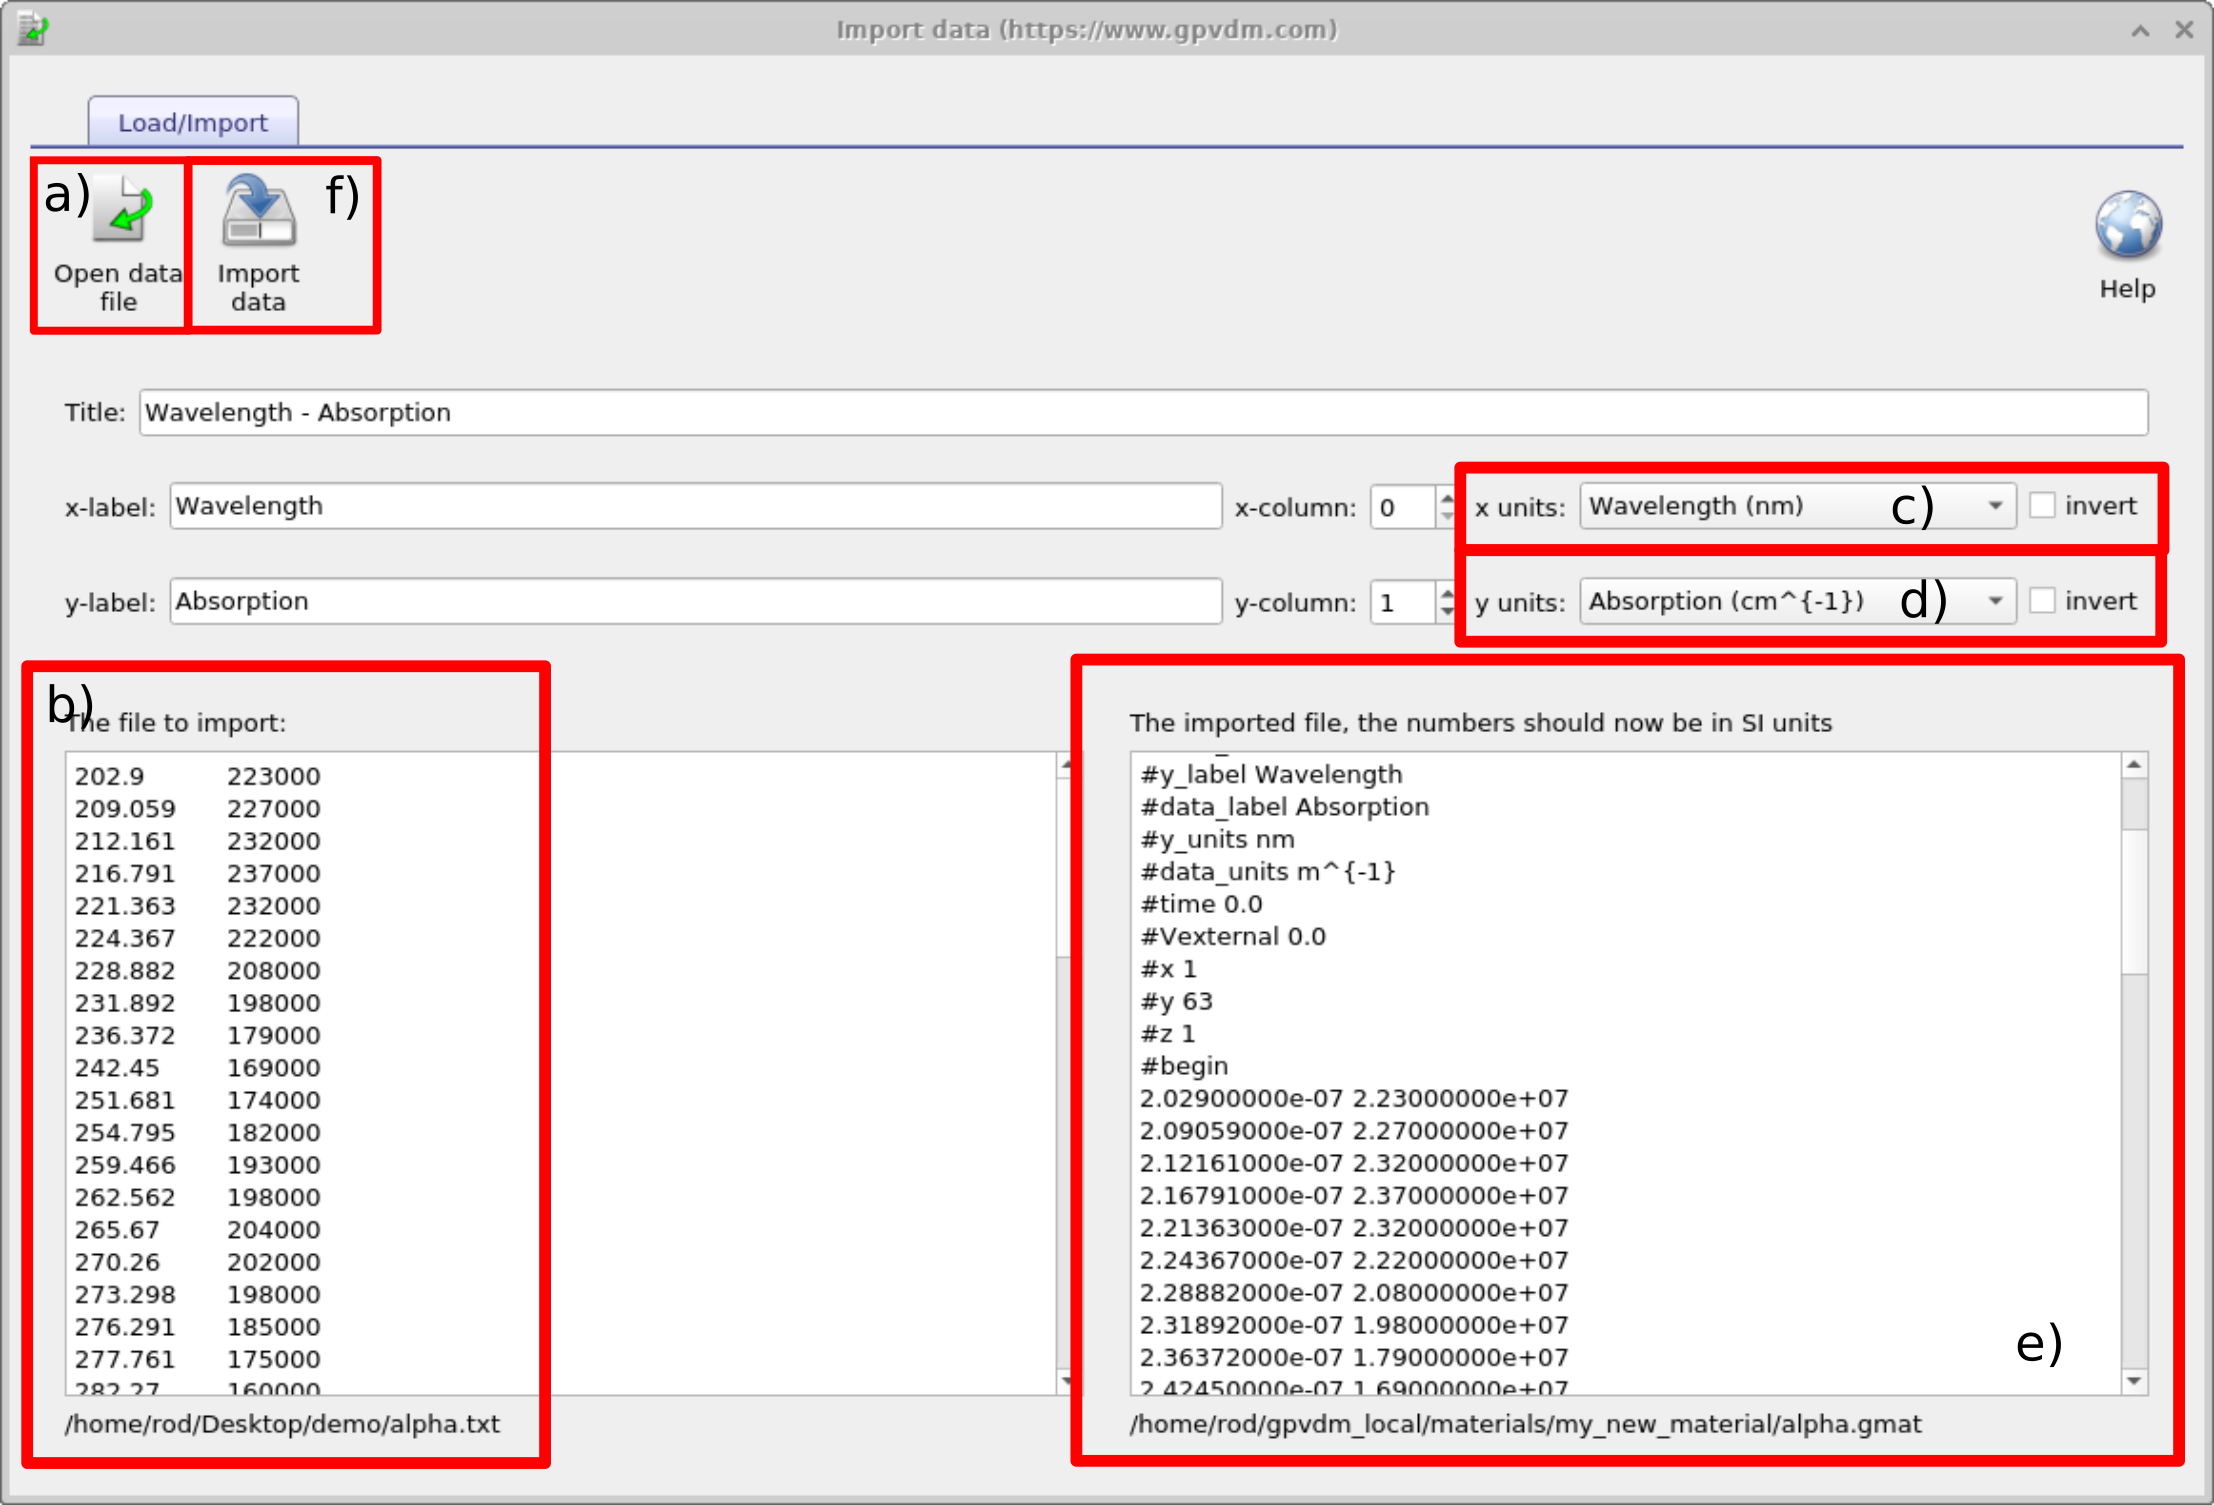
\includegraphics[height=0.7\textwidth]{./images/database_materials/database_import_window.png}
\caption{The data importer window}
\label{fig:materialadd6}
\end{figure}

\begin{figure}
\centering
\begin{tabular}{ c c }

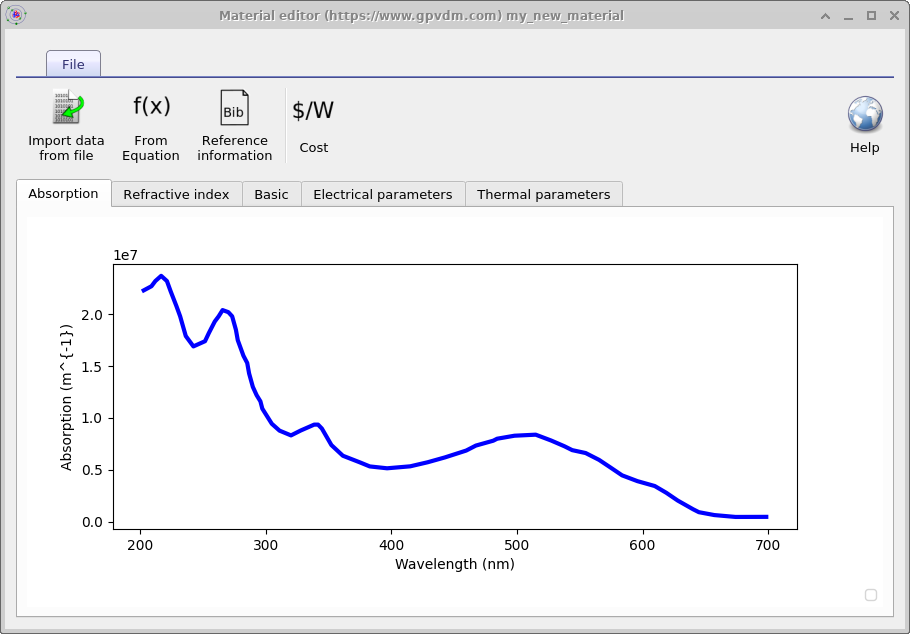
\includegraphics[width=0.5\textwidth,height=0.4\textwidth]{./images/database_materials/database_final.png}

&
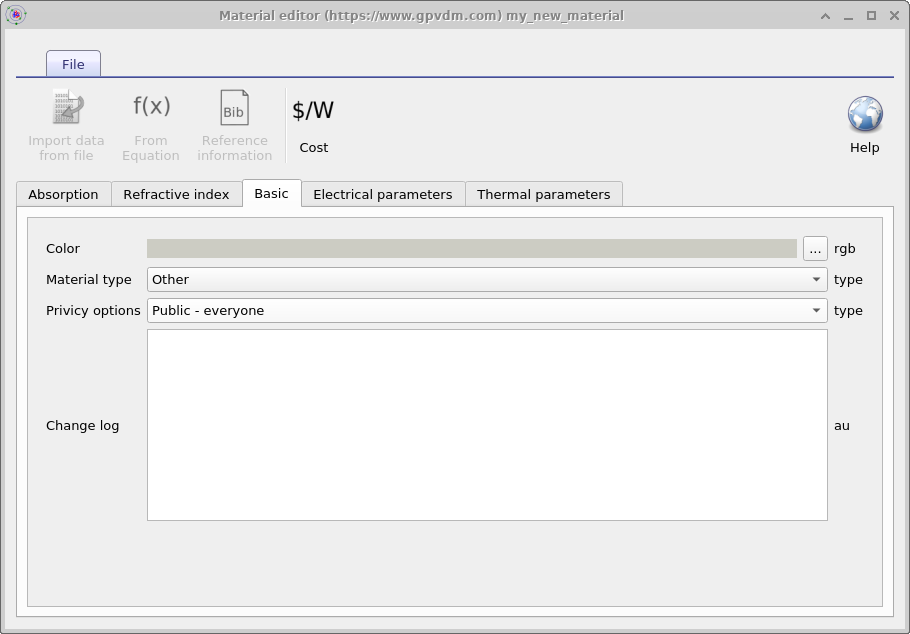
\includegraphics[width=0.5\textwidth,height=0.4\textwidth]{./images/database_materials/database_material_basic.png}
\\

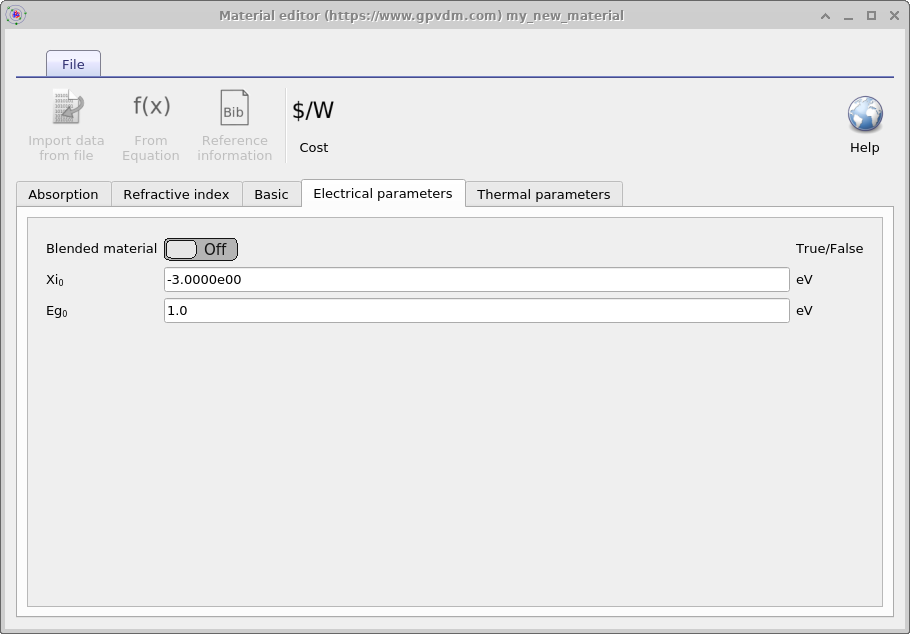
\includegraphics[width=0.5\textwidth,height=0.4\textwidth]{./images/database_materials/database_electrical_parameters.png}

&
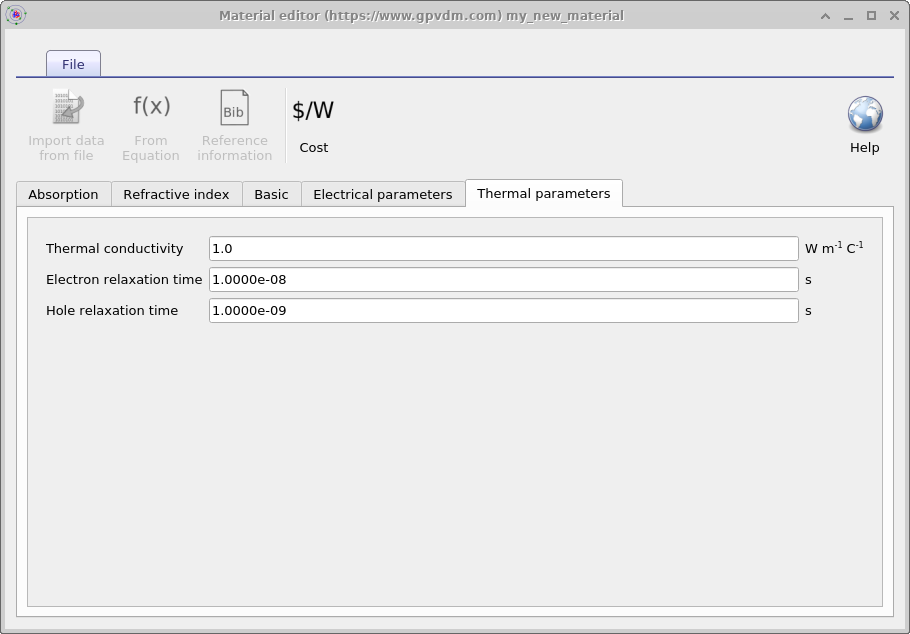
\includegraphics[width=0.5\textwidth,height=0.4\textwidth]{./images/database_materials/database_thermal_params.png}
\\
\end{tabular}
\caption{Clockwise from the top left; The imported absorption spectra; The basic material parameters; The electrical parameters; and the Thermal parameters.}
\label{fig:materialadd7}
\end{figure}

\newpage
\subsection{But I have a data in nm/n/k format}
Usually OghamNano only accepts data input in SI units and usually only accepts input in one format. This is to reduce the overall number of lines of code and reduce maintenance. However, I have been asked to make the model accept data of format: wavelength (nm), refractive index (au), k (au), as shown in Figure \ref{fig:wavelength_n_k}. OghmaNano will be able to read this file if you simply copy it into your\_home\_directory$\backslash$oghma\_local$\backslash$materials and give it a file extension .nk, so for example ito.nk.  Where your\_home\_directory is simply your Windows home directory. It is usually located on the C:$\backslash$Users on a home PC but the location can change if you are on a corporate PC. Once you have dragged the file into your\_home\_directory$\backslash$oghma\_local$\backslash$materials it will appear as a material in the model. See Figure \ref{fig:nk_file}. You can see that the .nk file in Figure \ref{fig:nk_file} is greyed out, this is because it is a non standard OghamNano file, that OghmaNano can read but not edit.

\begin{figure}[H]
\centering
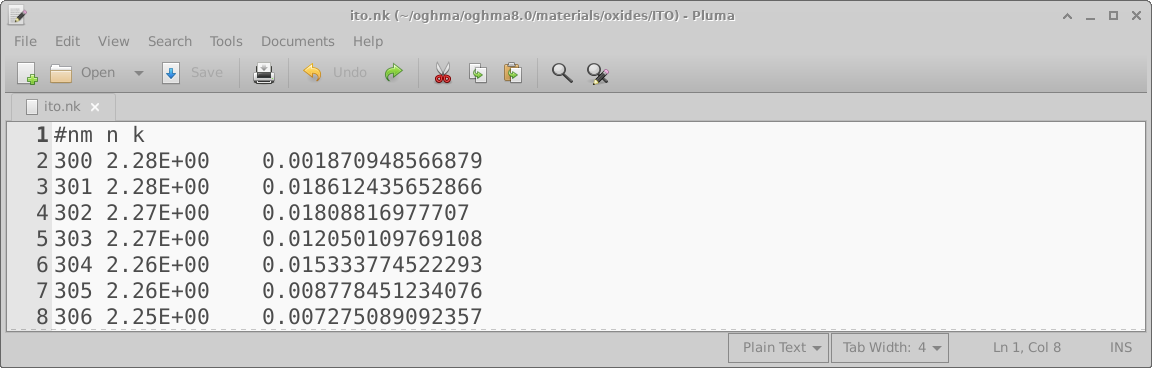
\includegraphics[width=0.7\textwidth]{images/database_materials/wavelength_n_k_example.png}
\caption{An example of wavelength/n/k data.}
\label{fig:wavelength_n_k}
\end{figure}

\begin{figure}[H]
\centering
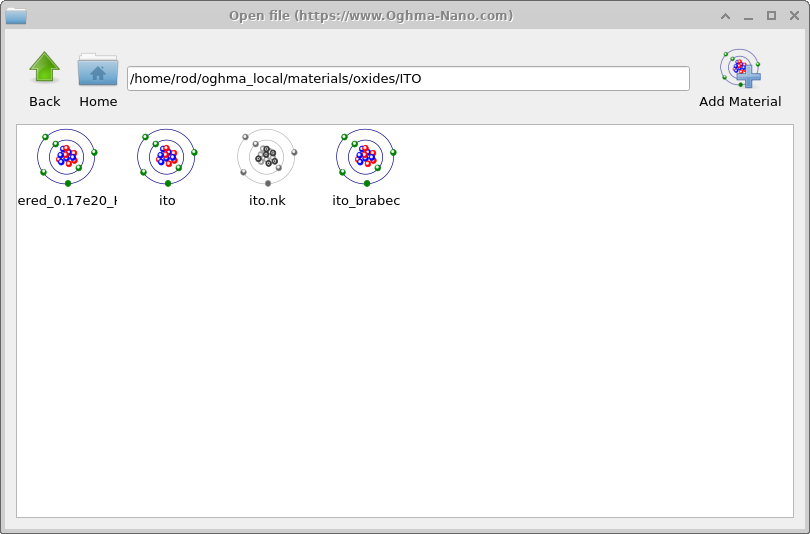
\includegraphics[width=0.7\textwidth]{images/database_materials/nk_file.png}
\caption{An example of a .nk file containing  wavelength/n/k data in the materials database.  You can see it is greyed out denoting that the file is not in native OghmaNano format.}
\label{fig:nk_file}
\end{figure}

\newpage
